
%(BEGIN_QUESTION)
% Copyright 2006, Tony R. Kuphaldt, released under the Creative Commons Attribution License (v 1.0)
% This means you may do almost anything with this work of mine, so long as you give me proper credit

Determine the pressure at each port of the DP transmitter during an instrument technician's step-by-step valve isolation procedure.  Assume the process fluid sensed by the transmitter is a gas and not a liquid:

$$\includegraphics[width=15.5cm]{i00026x01.eps}$$

% No blank lines allowed between lines of an \halign structure!
% I use comments (%) instead, so that TeX doesn't choke.

$$\vbox{\offinterlineskip
\halign{\strut
\vrule \quad\hfil # \ \hfil & 
\vrule \quad\hfil # \ \hfil & 
\vrule \quad\hfil # \ \hfil \vrule \cr
\noalign{\hrule}
%
% First row
Step & High-side pressure & Low-side pressure \cr
%
\noalign{\hrule}
%
% Another row
1: Transmitter in service &  &  \cr
%
\noalign{\hrule}
%
% Another row
2: Close high-side block valve &  &  \cr
%
\noalign{\hrule}
%
% Another row
3: Close low-side block valve &  &  \cr
%
\noalign{\hrule}
%
% Another row
4: Open equalizing valve &  &  \cr
%
\noalign{\hrule}
%
% Another row
5: Open bleed valve &  &  \cr
%
\noalign{\hrule}
} % End of \halign 
}$$ % End of \vbox

Based on the process pressures shown, identify the direction of process gas through this heat exchanger.

\vskip 10pt

Also, identify what the technician needs to tell the process operator(s) prior to isolating the transmitter from this process.

\vfil

\underbar{file i00026}
\eject
%(END_QUESTION)





%(BEGIN_ANSWER)

This is a graded question -- no answers or hints given!

%(END_ANSWER)





%(BEGIN_NOTES)

When the equalizing valve is opened {\it after} both block valves are shut, the pressures between the two sides of the transmitter's sensing capsule will tend to average each other.  Thus, 735 PSI trapped on the high side and 729 PSI trapped on the low side will become approximately 732 PSI on both sides after the equalizing valve is open:

% No blank lines allowed between lines of an \halign structure!
% I use comments (%) instead, so that TeX doesn't choke.

$$\vbox{\offinterlineskip
\halign{\strut
\vrule \quad\hfil # \ \hfil & 
\vrule \quad\hfil # \ \hfil & 
\vrule \quad\hfil # \ \hfil \vrule \cr
\noalign{\hrule}
%
% First row
Step & High-side pressure & Low-side pressure \cr
%
\noalign{\hrule}
%
% Another row
1: Transmitter in service & 735 PSI & 729 PSI \cr
%
\noalign{\hrule}
%
% Another row
2: Close high-side block valve & 735 PSI & 729 PSI \cr
%
\noalign{\hrule}
%
% Another row
3: Close low-side block valve & 735 PSI & 729 PSI \cr
%
\noalign{\hrule}
%
% Another row
4: Open equalizing valve & 732 PSI & 732 PSI \cr
%
\noalign{\hrule}
%
% Another row
5: Open bleed valve & 0 PSI & 0 PSI \cr
%
\noalign{\hrule}
} % End of \halign 
}$$ % End of \vbox

One way to envision the equalization of pressures at step \#4 is to imagine what would happen if two car tires pumped up to different air pressures were connected together through a tube.  Since Pascal's Principle tells us any pressurized fluid in an enclosed volume will tend to distribute pressure equally throughout, the air molecules in the high-pressure tire will flow through the tube and into the low-pressure tire in order to equally distribute pressure, thus depleting the high-pressure tire of some air while adding some air to the low-pressure tire.  In the end, the pressures in both tires will be equal, and that pressure value will be somewhere between the two original tire pressures.

\vskip 10pt

The flow of process gas through this heat exchanger is {\it in} at the top and {\it out} at the bottom.  You can think of this in terms of voltage drop across a resistor in a DC electric circuit: potential is always greatest (i.e. most positive) where current (conventional flow notation) enters.

\vskip 10pt

Before isolating the transmitter from this process, the technician needs to alert the operator that the transmitter will be coming out of service.  In preparation for this, any controller depending on this transmitter for its process variable (PV) must be placed in manual mode, and operators will have to look at some other pressure-indicating instrument in order to manually control the pressure drop while the transmitter is out of service.  Also, any process alarms triggered by this transmitter's signal should be disabled so that nuisance alarms aren't generated when the technician takes it out of service.

%INDEX% Measurement, pressure: 3-valve manifold operation
%INDEX% Process: heat exchanger pressure drop measurement (generic)

%(END_NOTES)


